\section{Results} 
To understand curiosity in animals we have become interested in curiosity in artificial life. This is because algorithmic curiosity can,

\begin{itemize}
\item solve sparse reward problems \cite{needed},
\item solve deceptive reward problems \cite{needed},
\item solve multi-objective problems \cite{needed},
\item lead to diverse skills that are
\item robust to instability and \cite{needed} 
\item robust to damage \cite{needed}.
\end{itemize}

This list is unusually broad for a learning algorithm. There is however no mathematics to let us understand this. 

So then what is curiosity? 

We define curiosity as an open-ended search to learn any information \cite{Kidd2015}. We assume this search should be efficient, and is motivated by value. What we would like is a way to describe these ideas mathematically, for any kind of learning algorithm. This is because curiosity depends on many different kinds of learning. In the broadest case, curiosity would then allow for any kind of learning. So this is the setting we have chosen. 

\subsection{Memory and learning} 
Any notion of information value seems to require that there must be a memory, $\Theta$, and a way to learn, $f$. For our general mathematical theory we will define memory as,

\begin{itemize}
\item A set of real valued numbers
\item Embedded in a finite space, with $N$ dimensions 
\item Closed and bounded
\end{itemize}

Let us then define learning in a matching way then. We say a learning function \textit{can be any function} which maps observations $x$ into memory. Using the function-arrow notation this kind of learning is denoted by, $f(x;\Theta) \rightarrow \Theta'$. Likewise a forgetting function \textit{can be any function} which inverts the memory, $f^{-1}(x;\ \Theta') \rightarrow \Theta$. 

So what are observations? It is convenient to assume that all observations are also embedded in a finite real space, $x \sim X \in \mathbb{R}^m$, as are actions $a \sim A \in \mathbb{R}^k$ and that rewards are positive real numbers, $R \in \mathbb(R^{+})$. 

In calling them ``observations'' we do not mean to imply they must arise from the senses. Observations could be internally generated from thought, or externally generated from the senses, or both in combination. Observations may contain action information, or they may not. Observations may contain reward information, or they may not. We have no preference and wish to accommodate all the different kinds of cognition \cite{needed}. % TODO -- huge citation dump

\subsection{Information value} 
Let us say we have a memory $\Theta$, which has been learned by $f$ over a history of observations, $[f(x_0; \Theta_0), f(x_1; \Theta_1), f(x_2; \Theta_2), \ldots]$. Can we measure how much value the next observation $f(x_t)$ should have? If there is such a measure $E$, we think it is reasonable to require that it have certain properties.

\begin{enumerate}
	\item $E$ should depend only on a memory, and what can be immediately learned. ($x$, $\Theta$, and $f$)
	\item An observation that is known completely, or cannot be learned, should have a value of 0. (If $\Delta \Theta = 0$, then $E=0$)
	\item $E$ should be non-negative because learning is never itself harmful. ($E \ge 0$)
	\item $E$ should increase monotonically with the change in memory. ($E \propto \Delta \Theta$)
	\item $E$ for the same observation should become decelerating in finite time. ($E \rightarrow 0$ as $t \rightarrow T^*$)
\end{enumerate}

These properties are in part inspired by Shannon's axioms for information theory, and in part found in the theories of information maximization, and information foraging \cite{needed}. What we have done is make their aspects which were implicit in their learning algorithms become explicit and independent of any kind of learning. This is important because anything we can prove this way must then be true for most practical learning algorithms \cite{MacKay2003}. 

We can satisfy all these by taking a geometric view of learning, as given in the definitions below. They are also shown graphically in Fig.~\ref{fig:cartoon} and described in detail in Boxes ~\ref{box:norm}-\ref{box:laplacian}.

\begin{itemize}
	\item[] \textbf{Definition 1} Let $E$ be the norm of $|| f_{\Theta}(x) - \Theta ||$.	
	\item[] \textbf{Definition 2} Let $|| f_{\Theta}(x)||$ be constrained such that $\nabla^2 \Theta < 0$ for all $ t \ge T^*$. 	
\end{itemize}

\begin{figure}
	\begin{fullwidth}
	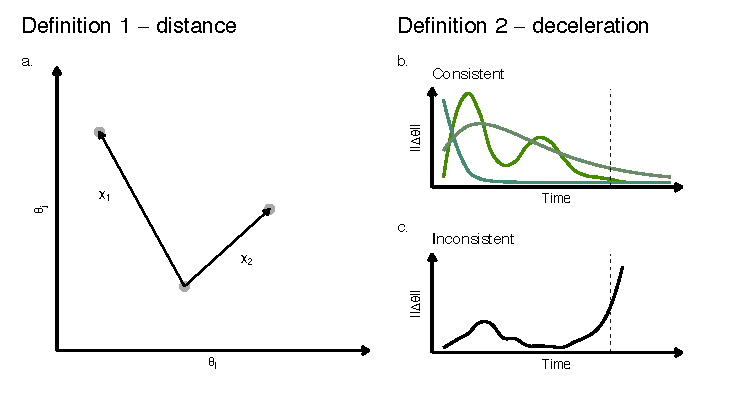
\includegraphics[width=0.7\linewidth]{img/cartoon.pdf} 
	\caption{A diagram of our definitions. 
	\textbf{a}. This panel illustrates a two dimensional memory. The information value of two observations $x_1$ and $x_2$ depends on the norm of memory with learning. Here we show this distance as a euclidean norm, denoted as a black arrow.
	\textbf{b-c} This panel illustrates learning dynamics with time (over a series of observations that are not shown). If information value becomes decelerating in finite time bound, then we say that learning is consistent with Def. 2. This is shown in panel b. The bound is depicted as a dotted line. If learning does not decelerate, then it is said to be inconsistent with Def. 2 (Panel c). \textit{It is important to note:} our account of curiosity does not apply when learning is inconsistent.
  	}
	\label{fig:cartoon} 
	% \figsupp{} % No limit on these.
	\end{fullwidth}
\end{figure}

% --------------------------------------------------------------------------
\begin{featurebox}
\caption{Norms.}
\label{box:norm}
A \textbf{norm} is a mathematical way to measure the overall size or extent of an ``object'' in a space. The object we are concerned with is a mathematical object with a form given by, $\Delta \Theta = f_{\Theta}(x) - \Theta$. But to define the norm let us as the first step consider a generic vector $v$. Keeping with convention will have its norm denoted by $||v||$, and defined by three properties:

\begin{enumerate}
  \item $||v|| > 0$ when $v \neq 0$ and $||v|| = 0$ only if $v=0$ (point separating)
  \item $||k v|| = ||k||\ ||v||$ (absolute scalability)
  \item $||v + w|| \leq ||v|| + ||w||$ (the triangle inequality)
\end{enumerate}

What does this mean for $\Delta \Theta$? A norm over a changing memory provides most the properties we require for our definition of $E$. It depends only on learning (and forgetting), that dependence must be monotonic, a norm is zero only when nothing in the space/memory changes and is positive definite. These satisfy the first four properties. For the fifth, see Box \ref{box:laplacian}.
\medskip
\end{featurebox}

\begin{featurebox}
	\caption{The Laplacian.}
	\label{box:laplacian}
	Here we use $\nabla^2$ to represent the \textbf{Laplacian}, which provides the second derivative of vector value functions \cite{needed}, giving us the remaining property we need. (See Box \ref{box:norm} for the others). To explain why, suppose we are working with a 1- dimensional memory. In this case the Laplacian reduces to the second derivative on our memory, $\frac{d^2\Theta}{dx^2} < 0$. A negative second derivative will force the changes in memory to be decelerating, by definition. In higher dimensions of memory then, a reader can think of the Laplacian as the ``second derivative'' of vector-valued functions like $f$. That is, negative Laplacian imply decelerating by definition.
	\medskip
\end{featurebox}
% --------------------------------------------------------------------------

% TODO clean this; need to end with concrete examples?
% We choose these definitions because their minimalism makes them extremely general, covering all modes of working or episodic memory (17, 18), probabilistic memory (19–21), count-based memory, predictive coding, and even memories based categorization, compression or latent-states (22, 23). 

\subsection{Exploration as a dynamic programming problem}
Curiosity is a search to maximize information value, again in the broadest sense possible. We decided to seek a dynamic programming solution to maximizing curiosity. This is useful because it would guarantee value is maximized, which, because of the way we have made our definitions, also guarantees that learning is complete. It is also convenient because dynamic programming is the basis for reinforcement learning \cite{Sutton2018}. 

The normal route to find a dynamic programming solution is to first prove your problem has ``optimal substructure'', then to derive the final result using Bellman optimality, and this is the route we will follow. For a more complete introduction to optimal substructure, see Box~\ref{box:substructure}. For more on dynamic programming and Bellman optimality, see Box~\ref{box:bellman}. 

In Theorem~\ref{theorem:opt_sub} (mathematical appendix) we prove our definition of memory has optimal substructure. This proof relies on the forgetting function $f^{-1}$ to succeed. Even though we have said little about it until now, this why we include forgetting in our early definitions. 

% -------------------------------------------------------------------------
\begin{featurebox}
	\caption{Dynamic programming and Bellman optimality.}
	\label{box:bellman}
	The goal of dynamic programming is to find a series of actions $(a_1, a_2, ..a_T)$, drawn from a set $A$, that maximize each payout $(r_1, r_2, ..., r_{T})$ so the total payout received is as large as possible. If there is a policy $a = \pi(x)$ to take actions, based on a series of observations $(x_0, x_1, ..x_{T}),$, then an optimal policy $\pi^*$ will always find the maximum total value $V^* = \argmax_{A} \sum_T r_t $. The question that Bellman and dynamic programming solve then is how to make the search for finding $\pi*$ tractable. In the form above one would need to reconsider the entire sequence of actions for any one change to that sequence, leading to a combinatorial explosion. 
	
	Bellman's insight was a way to make the problem simpler, and break it down into a small set of problems that we can solve in a tractable way without an explosion in complexity. This is his principle of optimality, which reads:

	\begin{quote}
		An optimal policy has the property that whatever the initial state and initial decision are, the remaining decisions must constitute an optimal policy with regard to the state resulting from the first decision. \cite{needed}
	\end{quote}

	Mathematically this allows us to translate the full problem, $V^* = \argmax_{\pi} \sum_T r_1, r_2, ..., r_{T}$ to a recursive one, which is given below. 

	\begin{equation}
		V^* = \argmax_{\pi} \ \Big [ r_0 + V(x_1) \ \Big ]
	\end{equation}
	
	Using this new form we can find an optimal solution by moving though the sequence of action iteratively, and solving each step independently. The question which remains though is how can we ensure our problem can be broken down this way? This is addressed in Box~\ref{box:substructure}.
	\medskip
\end{featurebox}
% -------------------------------------------------------------------------

% -------------------------------------------------------------------------
\begin{featurebox}
	\caption{Optimal substructure}
	\label{box:substructure}
	To use Bellman's principle of optimality (Box~\ref{box:bellman}) the problem we want to solve needs to have \textbf{optimal substructure}. This opaque term can be understood by looking in turn at another theoretical construct, Markov spaces. 
	\\
	In Markov spaces there are a set of states or observations $(x_0, x_1, ..., x_{T})$, where the transition to the next $x_t$ depends only on the previous state $x_{t-1}$. This limit means that if we were to optimize over these states, as we do in reinforcement learning, we know that we can treat each transition as its own ``subproblem'' and therefore the overall situation has ``optimal substructure''.
	\\
	In reinforcement learning the problem of reward collection is defined by fiat as happening in a Markov space \cite{Sutton2018}. The problem for curiosity is it relies on memory and memory, being necessarily composed of many past observations in many orders, cannot be a Markov space. So if we wish to use dynamic programming to maximize $E$, we need to find another way to establish optimal substructure. This is the focus of Theorem~\ref{theorem:opt_sub}.
	\medskip
\end{featurebox}
% -------------------------------------------------------------------------

The Bellman derivation leads to an especially practical and simple result (Eq. \ref{eq:V_E}). Given an arbitrary starting value $E_0 > 0$, the dynamic programming solution to maximizing $E$ is given by Eq. ~\ref{eq:V_E_bellman}. A full derivation is provided in the mathematical appendix. We denote our policy that follows this solution as $\pi_E$.

\begin{equation}
	\label{eq:V_E_bellman} 
	V^{\pi}_E(x) = \argmax_A \Big [ E_0 + V_E(x_1) \Big ]
\end{equation}


However as long as the search for $E$ continues until learning is at a steady-state, and as result information value is zero, then there are a range of equally good solutions (Theorem \ref{TODO}). These let us simplify Eq. \ref{eq:V_E_bellman} further, giving Eq. \ref{eq:EE}. 

\begin{equation}
	\label{eq:EE} 
	V^{\pi}_E(x) = \argmax_A \Big [ E_0 + E(x_1) \Big ]
\end{equation}

\subsection{Optimal exploration, and the importance of boredom}
In our opening we said curiosity is a search for information, but we also said it should be an efficient search. So what would it mean for a curiosity search  to be efficient? Does our Bellman solution ensure it?

We have discussed maximizing curiosity by means of $E$ but to study efficiency we must now discuss limiting it. This is necessary because exploration is limited in practice by the available energy, hunger, greed, thirst or other biological priorities. But more importantly search must be limited to avoid the central limit of curiosity: it can become distracted by minutia. A good example of minutia was given \cite{Pathak2017} who asks us to, ``Imagine a scenario where the agent is observing the movement of tree leaves in a breeze. Since it is inherently hard to model breeze, it is even harder to predict the location of each leaf''. This will imply, they note, that a curious agent will always remain curious about the leaves, to its own detriment. 

The solutions to both problems are the same. To limit curiosity we will draw on its opposite, boredom \cite{Schmidhuber1991}. Others have considered boredom an adaptive trait as well, arguing it is a useful way to motivate aversive tasks \cite{Bench2013}. We take a slightly different view and consider boredom as a means to ignore the marginal, and as a tunable free parameter, $\eta \ge 0$. That is, we say curious exploration should cease once $E$ becomes marginal as given by Eq.~\ref{eq:null}. 
\begin{equation}
	\label{eq:null}
	E \le \eta : \pi_E \rightarrow \pi_{\emptyset}
\end{equation}

Here we use $\pi_{\emptyset}$ to denote any other action policy that is not $\pi_E$. Informally what Eq.~\ref{eq:null} means is that once $E$ is below the boredom threshold, E is marginal, and the learner should change its behavior from exploration to some other policy. This change in behavior could be towards an aversive policy (as in \cite{Bench2013}) or it could be towards reward seeking, as we will assume.

We think it is reasonable to call a curious search optimal if it meets the three criteria below. In Theorem~\ref{needed} we prove that $\pi_E$ satisfies these, when $\eta > 0$.

\begin{enumerate}
	\item Exploration should visit all available states of the environment at least once.
	\item Exploration should cease when learning has plateaued.
	\item Exploration should take as few steps as possible to achieve 1 and 2.
\end{enumerate}

\subsection{The importance of determinism in search}
The work so far has built up the idea that the most valuable, and most efficient, curious search will come from a deterministic algorithm. That is, every step strictly maximizes $E$. It is also this determinism which will let us resolve the dilemma, later on. A deterministic view of exploration is at odds with how the problem is generally viewed today, which involves some amount of randomness. Whereas if our analysis is correct, randomness is not needed or desirable, as it must lead to less value and a longer search. We confirm and illustrate this result using an exmple of a simple information foraging task (Fig.\label{fig:task_outline}\textbf{a}). The results of which are shown in Figure~\ref{needed}. 

Besides offering a concrete example, performance in this Task 1 is a first step in showing that even though $\pi_E$'s optimality is proven for a deterministic environment in our proofs, it will perform well if not optimal in stochastic settings.

\begin{figure}
	\begin{fullwidth}
	\includegraphics[width=.4\linewidth]{img/task_outline.pdf} 
	\caption{The two basic kinds of tasks we will study.	
\textbf{a.} Represents a very simple information foraging task. The information is a yellow or blue stimulus, which can change probabilistically from trial to trial. A good learner in this task is one who tries to learn the probabilities of all the symbols in each of the four choices. The more random the stimuli are in a choice, the more potential information/entropy there is to learn.  
	\textbf{b.} Represents a very simple reward collection task. The reward is numerical value, here a 1 or 0. A good learner in this task is one who collects the most rewards.}
	\label{fig:task_outline} 
	\end{fullwidth}
\end{figure}

\begin{figure}
	\begin{fullwidth}
	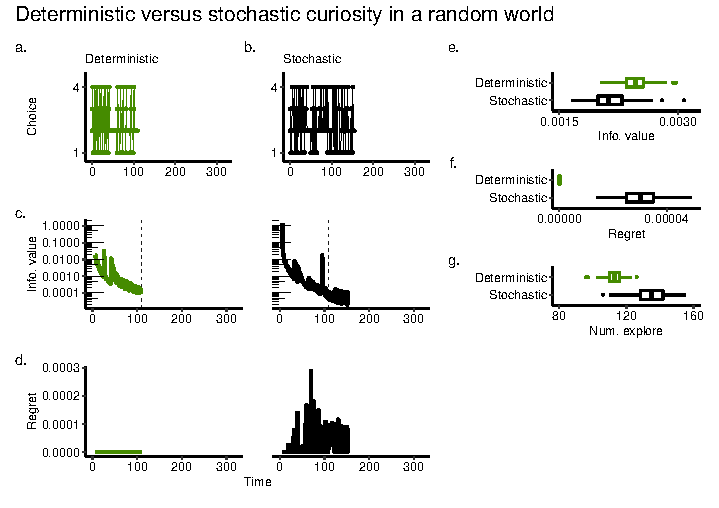
\includegraphics[width=.6\linewidth]{img/curiosity1.pdf} 
	\caption{Comparing deterministic and stochastic curiosity in a simple information foraging task (Task 1). Deterministic results are shown in the left column, and stochastic are shown in the right. The hyperparameters for both models were found by random search, which is described in the Methods.
	\textbf{a-b}. Examples of choice behavior.
	\textbf{c-d}. Information value plotted with time for the behavior shown in a-b.
	\textbf{e-f}. Regret plotted with time for the behavior shown in a-b. Note how our only deterministic curiosity generates zero regret, inline with theoretical predictions.
	\textbf{e}. Average information value for 100 independent simulations. Large values mean a more efficient search.
	\textbf{f}. Average regret for 100 independent simulations. Ideal exploration should have no regret. 
	\textbf{g}. Number of steps it took to reach the boredom threshold $eta$. Smaller values imply a faster search.
	}
	\label{fig:curiosity1} 
	\end{fullwidth}
\end{figure}

\subsection{The dilemma}
How can we justify using curiosity for the dilemma problem when the goal of exploitation is reward collection? Intuition suggests that searching for in an open-ended way must be less efficient than a direct search. We have an answer in two conjectures:

\begin{itemize}
	\item \textbf{Conjecture 1} Reward value and information value are equally important.
	\item \textbf{Conjecture 2} Curiosity is a sufficient solution to exploration (when learning is the goal)
\end{itemize}

If reward and information are equally important, how can an animal go about balancing them? We will argue that answering this question is the same as answering the exploration-exploitation dilemma. So can we solve the dilemma with independent policies? 

We will answer this last question using the framework of regret minimization, which is the standard view. Regret is a numerical quantity that represents the difference between the most valuable choice, and the value of the choice that was made. To approximate regret $G$ we use Eq. \ref{eq:regret}, where $V$ is the value of the chosen action, and $V^*$ is the maximum value. 

\begin{equation}
\label{eq:regret}
	G = V^* - V
\end{equation}

An optimal value algorithm with zero regret always makes the most valuable choice. But this is impossible to achieve when exploring any dynamic or uncertain environment using stochastic search. 

To find the algorithm that maximizes both information and reward value with zero regret, we imagined the policies for exploration and exploitation acting as two possible ``jobs'' competing for control of behavior, a fixed resource. We know (by definition) each of these jobs produces non-negative values which an optimal job scheduler could use: $E$ for information or $R$ for reward/reinforcement learning. We can also ensure (by definition) that each of the jobs takes a constant amount of time and that each policy can only take one action at a time. These two properties, and one further assumption, are sufficient.

We believe it is reasonable to assume that there will be no model of the environment available to the learner at the start of a problem, and that its environment is nonlinear but deterministic. 

We arrived at our solution by taking the simplest possible path available. We just wrote down the simplest equation that could have zero regret answer, and began to study that. This is Eq.~\ref{eq:meta_greedy}. We refer to it as a meta-greedy algorithm, as it decides in greedy fashion which of our independent policies to use.

\begin{equation}
\label{eq:pipi} 
\pi^{\pi} = \ \Big [ \pi_E,\ \pi_R \Big ]
\end{equation}

\begin{equation}
\label{eq:meta_greedy} 
	\argmax_{\pi^{\pi}} \ \Big [ E_{t-1},\ R_{t-1} \Big ]_{\textbf{(2, 1)}}
\end{equation}
	
We have in Eq. \ref{eq:meta_greedy} modified traditional argmax notation. It now includes a vector $(2,1)$ to denote a ranking system for which value/policy should be preferred in the event of a tie. Smaller numbers are more preferred. We add this notation because an exact rule for tie breaking is critical to our mathematical proofs (which follow below). 

In Eq. \ref{eq:meta_greedy} we also limit the probability of having zero reward to be, itself, non-zero. That is, $p(R_t=0) > 0$. This is necessary to ensure exploration. For reasons of mathematical convenience we also limit $E_t$ to be positive and non-zero when used with boredom, $(E_t - \eta) \geq 0$. 

In Theorem \ref{theorem:meta_total} we prove Eq. \ref{eq:meta_greedy} is Bellman optimal, and so it will always find a maximum value sequence of $E$ and $R$ values. Given, that is, an initial value $E_0 > 0$, and that the environment is deterministic. In Theorem \ref{theorem:meta} we also prove that with a judicious choice in boredom $\eta$, the reward policy $\pi_R$ will also converge to its optimal value, assuming it has one. For full details the mathematical appendix.

% PUT IN TIT-FOR-TAT AND MENTION WIN-STAY LOSE-SHIFT.
Another way to think independent policies and Eq. \ref{needed} is as a animal playing a game of tit-for-tat against the past. Tit-for-tat is the strategy is famous game theory result, where a play mirrors their opponent’s actions. We see the same kind of pattern as useful here, except the opponent is simply the animal’s own past decisions. That is, if there was more reward value then information value on the last turn (action), then choose the reward policy this time or if more information value was found last time, then choose the information policy this time.

% -------------------------------------------------------------------------
\begin{featurebox}
	\caption{Algorithmic run time.}
	\label{box:complexity}
	It is common in computer science to study the runtime of an algorithm. So what is the runtime of our independent policies solution? There is unfortunately no fixed answer for the average or best case. The worst case algorithmic run time is linear and additive in the independent policies. If it takes $T_E$ steps for $\pi_E$ to converge, and $T_R$ steps for $\pi_R$, then the worst case run time for $\pi_{\pi}$ is $T_E + T_R$. 
	\medskip
\end{featurebox}
% -------------------------------------------------------------------------

% -------------------------------------------------------------------------
\begin{featurebox}
	\caption{Reward homeostasis.}
	\label{box:complexity}
	We have been studying a kind of reinforcement learning where the value of a reward is fixed. We'll call this the economic style. It is the most common kind of model found in machine learning, psychology, neuroeconomics, and neuroscience \cite{Sutton2018}. In natural behavior though it is common that the motivational value of reward declines as the animal gets ``full'', or reaches satiety. We'll call this the homeostatic style \cite{Keramati2014,Juechems2019,Munch2020}
	Fortunately it has already been proven that a reward collection policy designed for one style will work for the other (at least this is so an infinite time-horizon \cite{Keramati2014}). However to use Eq. \ref{eq:meta_greedy} for reward homeostasis requires we must make one intuitive modification. Ties between values should be broken in favor of exploration, and information seeking. (In the economic reinforcement learning ties break in favor of exploiting rewards). This modification leads to Eq. \ref{eq:meta_greedy_h}.

	\begin{equation}
		\label{eq:meta_greedy_h} 
			\argmax_{\pi^{\pi}} \ \Big [ E_{t-1},\ R_{t-1} \Big ]_{\textbf{(1, 2)}}
		\end{equation}
	\medskip
\end{featurebox}
% -------------------------------------------------------------------------

\subsection{Simulations of reward collection} We will now focus on practical performance, believing it is a compelling way to make the case for curiosity as sufficient. The general form of the 7 tasks we will study is depicted in Fig~\ref{fig:task_outline}. They are all variations of the classic multi-armed bandit \cite{Sutton2018}. The payouts for each are shown in Fig.~\ref{fig:payout1}-\ref{fig:payout2}. 

Each task was designed to either test exploration performance in a way that matches recent experimental study(s), or to test the limits of curiosity. On each trial was with a set of $n$ choices. Each choice returns a “payout”, according to a predetermined probability. Payouts are information, reward, or both (Fig.~\ref{fig:task_diagram}). Note that information was symbolic, denoted by a color code, “yellow” and “blue” and as is custom reward was a positive real number. A summary for each task, and a visual depiction of its payouts, are shown in Fig ~\ref{fig:payout}.

We have chosen a range of other exploration strategies to compare against. We feel it is broad enough that we have made a fair representation of today's state of the art. They are drawn from both neuroscience, and machine learning. They have in common that their central design goal was to maximize reward value, often supplemented by some other goal. For a brief description of each, see Table~\ref{tab:agents}. The results in full for all tasks and exploration strategies are shown in Fig.~\ref{fig:summary}. Note that all learners, including ours, used the same exploitation policy, based on the temporal difference learning rule \cite{Sutton2018,needed}.

\begin{figure}
	\begin{fullwidth}
	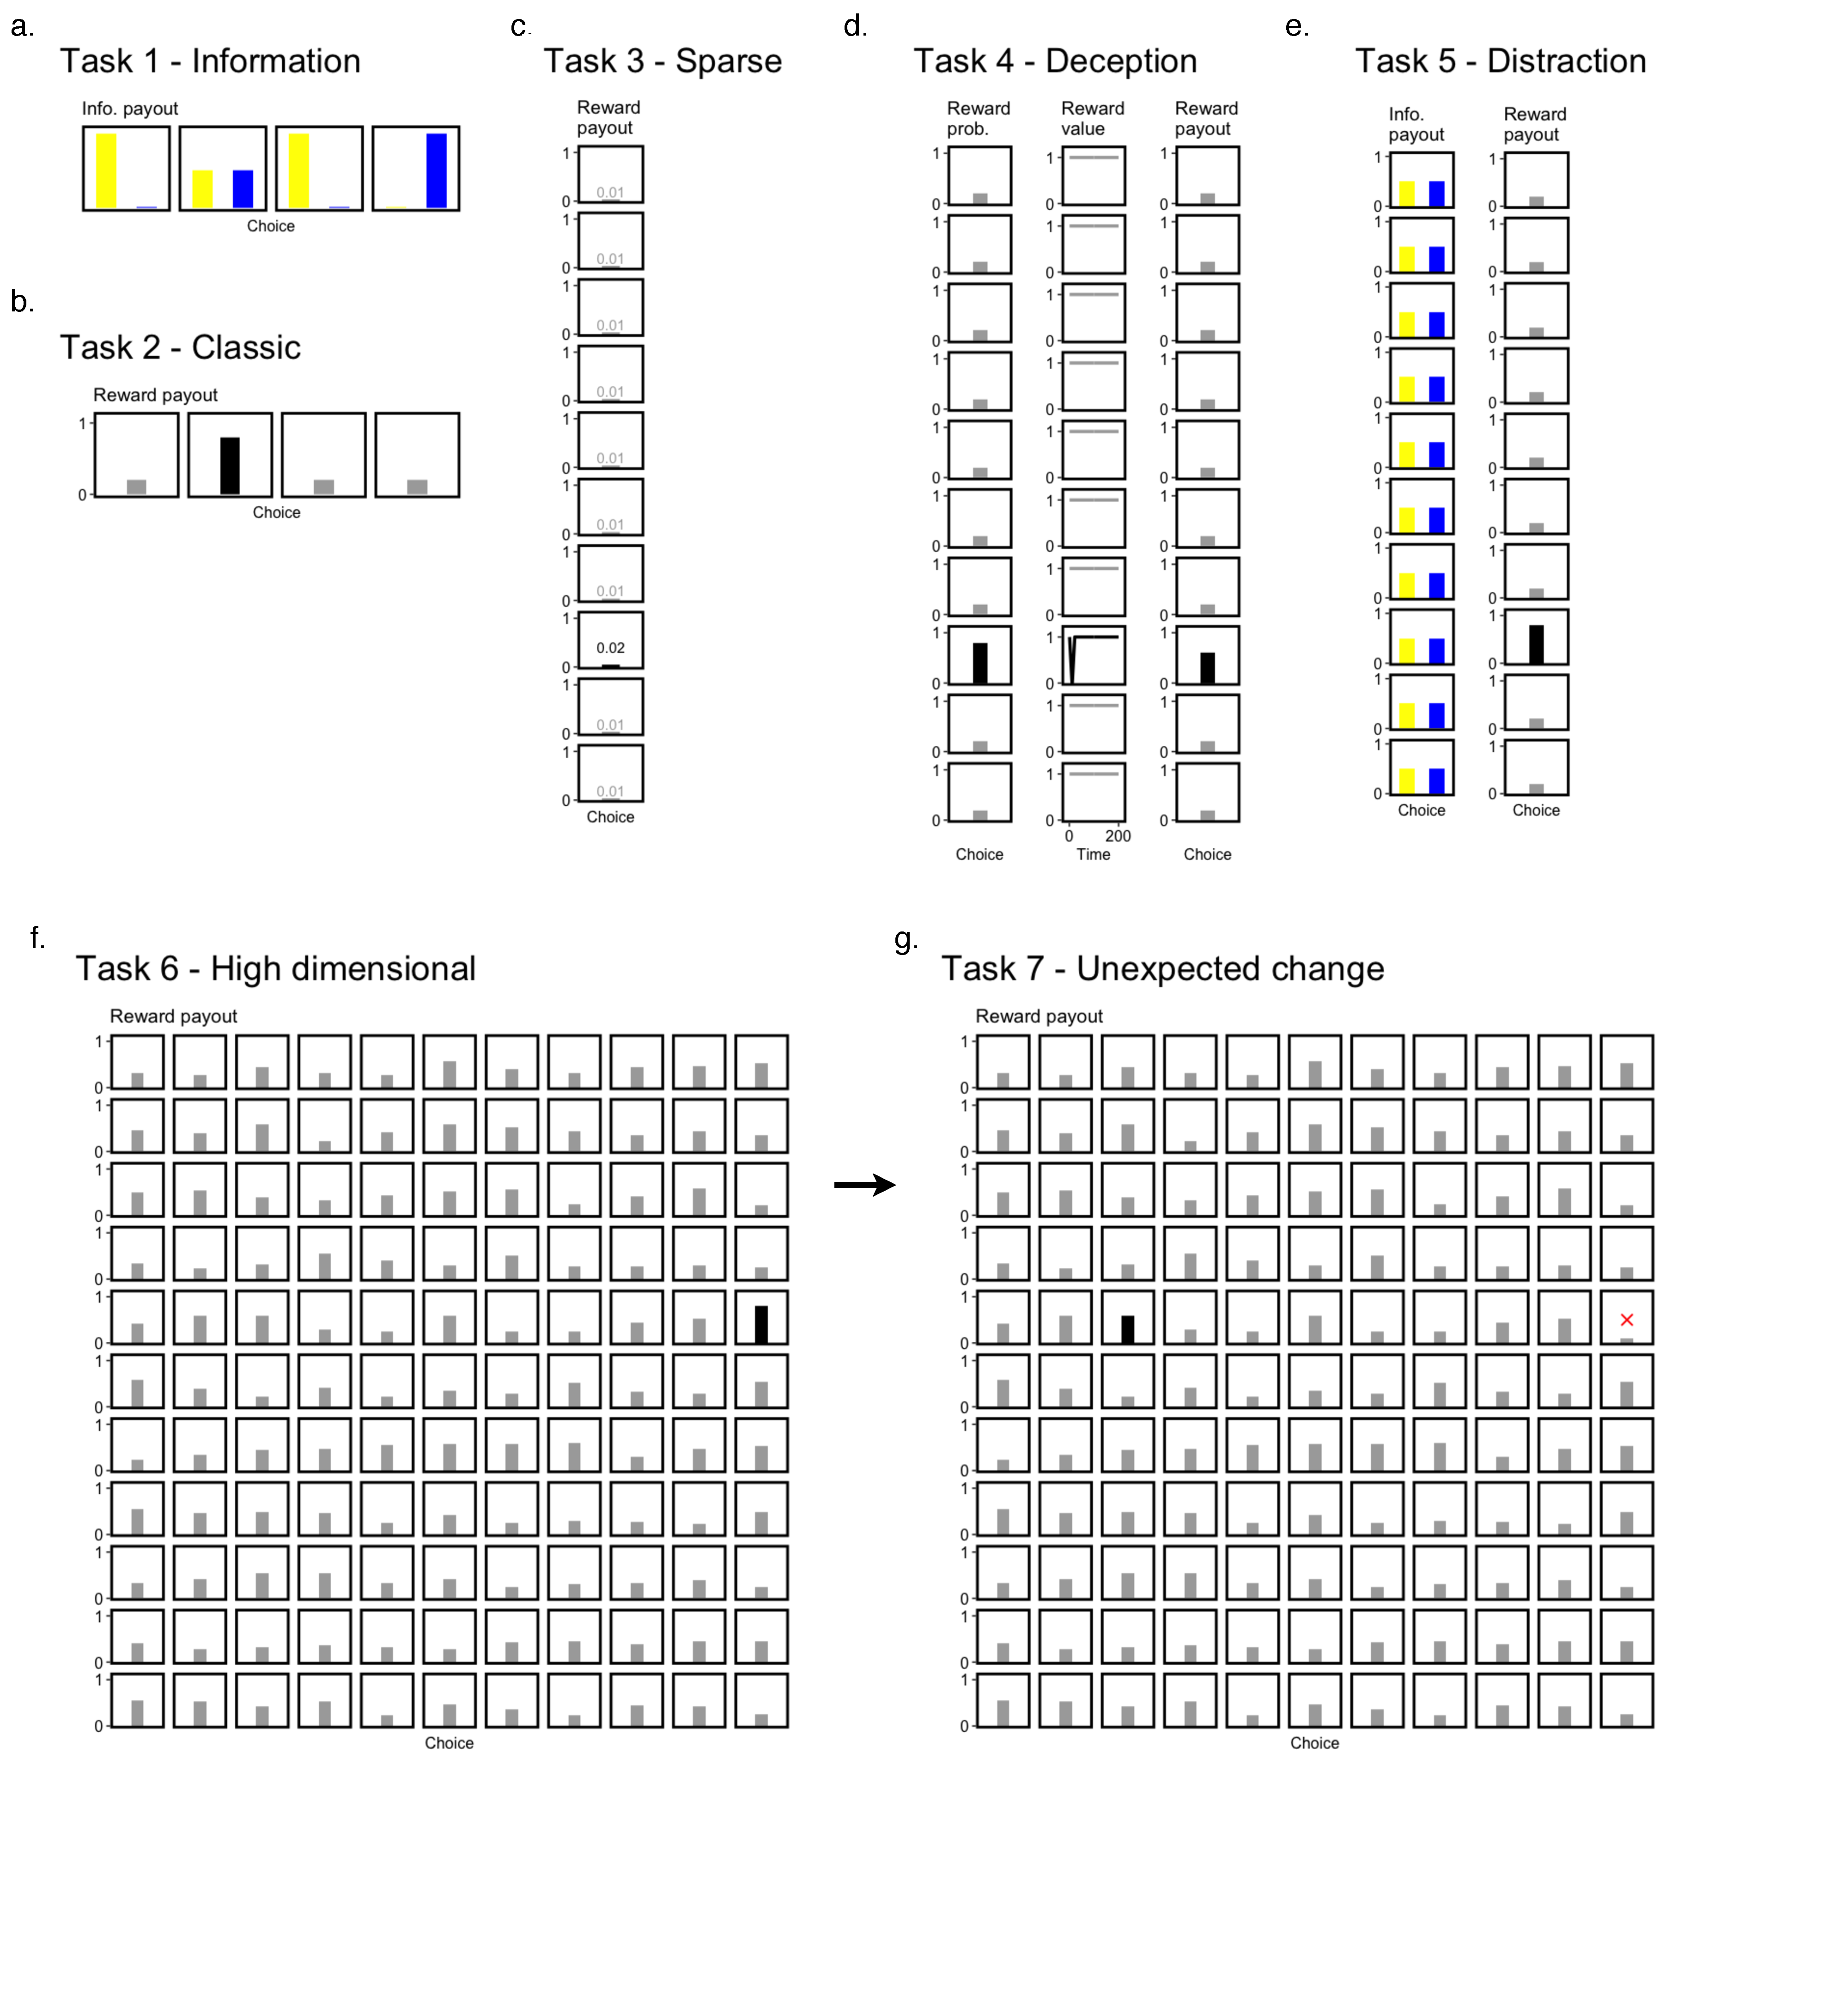
\includegraphics[width=.8\linewidth]{img/task_payout.pdf} 
	\caption{Payouts for \textit{Tasks 1 - 5}. Payouts can be information, reward, or both. For comments on general task design, see Fig~\ref{fig:task_outline}.
	\textbf{a.} A classic four-choice design for information collection. A good learner should visit each arm, but quickly discover that only arm two is information bearing.
	\textbf{b.} A classic four-choice design for testing exploration under reward collection. The learner is presented with four choices and it must discover which choice yields the highest average reward. In this task that is Choice 2. 
	\textbf{c.} A ten choice sparse reward task. The learner is presented with four choices and it must discover which choice yields the highest average reward. In this task that is Choice 8 but the very low overall rate of rewards makes this difficult to discover. Solving this task with consistency means consistent exploration. 
	\textbf{d.} A ten choice deceptive reward task. The learner is presented with 10 choices, but the choice which is the best on the long-term (>30 trials) has a lower value in the short term. This value first declines, then rises (see column 2).
	\textbf{e.} A ten choice information distraction task. The learner is presented with both information and rewards. A good learner though will realize the information does not predict reward collection, and so will ignore it.
	\textbf{f.} A 121 choice task with a complex payout structure. This task is thought to be at the limit of human performance. A good learner will eventually discover choice number 57 has the highest payout.
	\textbf{g.} This task is identical to \textit{a.}, except for the high payout choice being changed to be the lowest possible payout. This task tests how well different exploration strategies adjust to simple but sudden change in the environment.
	}
	\label{fig:payout} 
	\end{fullwidth}
\end{figure}

\begin{table}[]
	\caption{Exploration strategies.}
	\label{tab:agents}
	\begin{tabular}{|l|l|l|}
	\hline
	\textbf{Name} & \textbf{Class} & \textbf{Exploration strategy} \\ \hline
	Curiosity & Deterministic & Maximize information value \\ \hline
	Random/Greedy & Random & \begin{tabular}[c]{@{}l@{}}Alternates between random exploration \\ and greedy with probability $\epsilon$.\end{tabular} \\ \hline
	Decay/Greedy & Random & \begin{tabular}[c]{@{}l@{}}The $\epsilon$ parameter \\ decays with a half-life $\tau$\end{tabular} \\ \hline
	Random & Random & Pure random exploration \\ \hline
	Reward & Extrinsic & Softmax sampling of reward value \\ \hline
	Bayesian & Extrinsic + Intrinsic & Sampling of reward value + information value \\ \hline
	Novelty & Extrinsic + Intrinsic & Sampling of reward value + novelty signal \\ \hline
	Entropy & Extrinsic + Intrinsic & Sampling of reward value + action entropy \\ \hline
	Count (EB) & Extrinsic + Intrinsic & Sampling of reward value + visit counts \\ \hline
	Count (UCB) & Extrinsic + Intrinsic & Sampling of reward value + visit counts \\ \hline
	\end{tabular}
\end{table}

\begin{figure}
	\begin{fullwidth}
	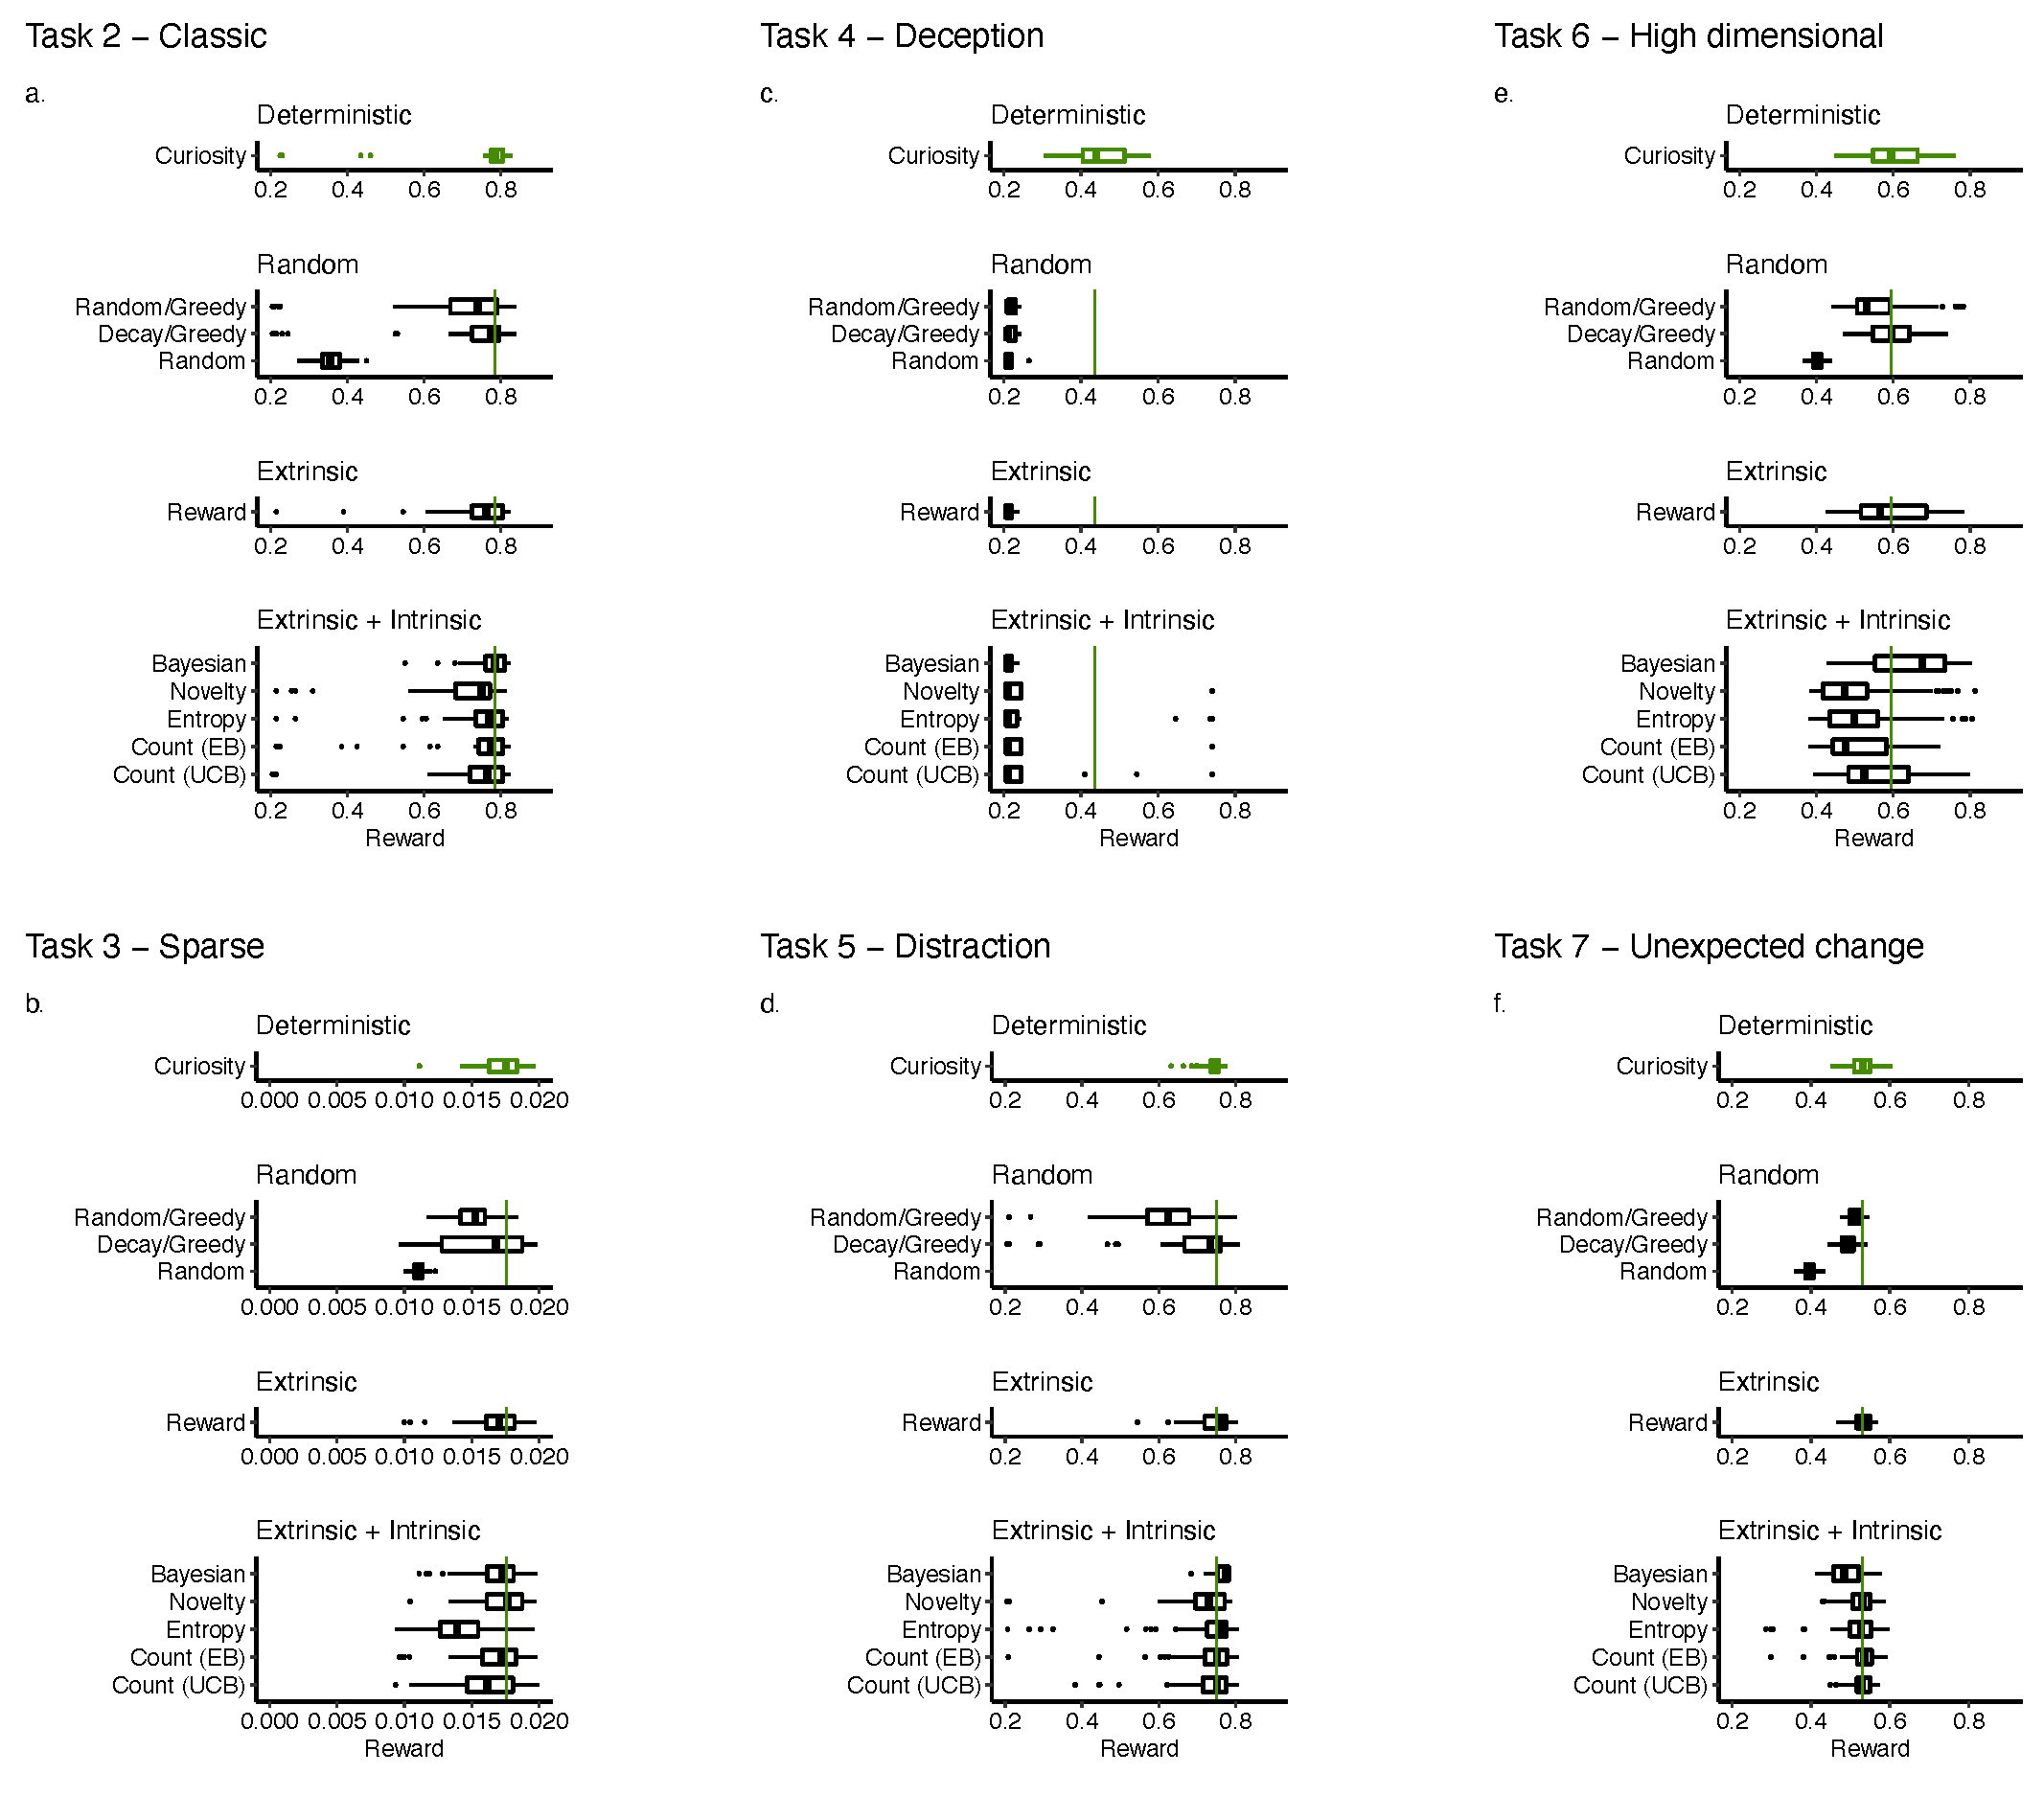
\includegraphics[width=1.1\linewidth]{img/summary.pdf} 
	\caption{Summary of reward collection (\textit{Tasks 2-7}). The strategies in each panel are grouped according to the class of search they employed (Curiosity. Random, Extrinsic reward or Extrinsic + Intrinsic rewards). 
	\textbf{a.} Results for Task 2, which has four choices and one clear best choice.
	\textbf{b.} Results for Task 3, which has 10 choices and very sparse positive returns.
	\textbf{c.} Results for Task 4, whose best choice is initially ``deceptive'' in that it returns suboptimal reward value over the first 20 trials.
	\textbf{d.} Results for Task 5, which blends the information foraging task 1 with a larger version of Task 2. The yellow/blue stimuli are a max entropy distraction which do not predict the reward payout of each arm.
	\textbf{e.} Results for Task 6, which has 121 choices and a quite heterogeneous set of payouts but still with one best choice.
	\textbf{f.} Results for Task 7, which is identical to Task 6 except the best choice was changed to be the worst. The learners from Task 6 were trained on this Task beginning with the learned values from their prior experience -- a test of robustness to sudden change in the environment. 
	\textit{Note}: To accommodate the fact that different tasks were run different numbers of trials, we normalized total reward by trial number. This lets us plot reward collection results for all tasks on the same scale.
  	}
	\label{fig:summary} 
	% \figsupp{} % No limit on these.
	\end{fullwidth}
\end{figure}

It is not possible for any one learning algorithm to work best in all situations \cite{needed}. A good outcome for our algorithm seems to be falling in the top 2 or 3 or so for all tasks. This is what we observed (Fig~\ref{fig:summary}). Given our aim to test our method of independent policies it is not interesting to detail the varieties of why performance was found to vary between strategies and tasks. The no free lunch theorem forbids any general no one strategy from prevailing on all problems \cite{needed}. 

In terms of curiosity's performance though its worth noting that on \textit{Task 4} ours is the only strategy that reaches above chance performance. This was then deception task, which was included to confirm that in a small amount deception derails exploration in the classic form and to confirm that our form of curiosity can overcome deception as we would expect it to 

In terms of curiosity, \textit{Task 5} is also worth a special note (Fig~\ref{fig:summary}\textbf{c}). It was designed to fool curiosity by presenting information that was irrelevant. What we saw though was that with judicious use of boredom, curiosity still produced a very high level of performance. In the supplementary figure we also show that if boredom is mistuned, curiosities performance suffers, but not catastrophically (TODO - add this figure). 

\textit{Tasks 6-7} are also worth noting (Fig~\ref{fig:summary}\textbf{e-f}). \textit{Task 6} was a 121 choice experiment that is at the limit of human performance \cite{needed}. In \textit{Task 7} then we had learning continue from Task 6, and all was the same except that what was the best choice in Task 6 was suddenly and unexpectedly was the worst choice in Task 7. Under this sudden nonstationarity the top strategy (Bayesian) became the worst, and curiosity took the top spot. (It was already second place in Task 6). This is exactly the kind of robustness we'd predict for any curiosity algorithm \cite{needed}. Curiosity drove an unbiased model of the value structure that allowed it to adapt quickly. As did it's worth noting all the other more unbiased exploitation models (the count, novelty, and entropy models; Fig~\ref{fig:summary}\textbf{f}).

When using Eq~\ref{eq:meta_greedy} a good choice of boredom $eta$ is critical, and was optimized carefully above. We show an example of this importance in Fig.~\ref{fig:boredom2} and in Fig~\ref{fig:task_outline}b. On the left hand side we did a random search over 10000 possible parameters to find a value for $\eta$ that produced excellent results. On the right hand side we choose a value for boredom we knew would lead to a relatively poor result. We then ran the 100 different randomly generated simulations which gives us the results seen in Fig.~\ref{fig:boredom2}). 

The optimized boredom converged far more quickly (Fig.~\ref{fig:boredom2}a-b), generating more reward over time (Fig.~\ref{fig:boredom2}c-d), and showed far more in consistency during exploration (Fig.~\ref{fig:boredom2}e-f). 

Fig.~\ref{fig:boredom2} is also useful in showing the wide variance in behavior which is possible with what is otherwise a deterministic search. That is, exploration in these figures is deterministic, as prescribed by Fig~\ref{needed}. What we see experimentally however is a wide range of behaviors (top panels), with very different distributions for their actions choices (bottom panels). This is no because exploration is stochastic, but can instead be understood by variations in the environment changing what is learned, which then changes what the best learner should choose to learn next. 

% TODO -- add exploration distributions
\begin{figure}
	\begin{fullwidth}
	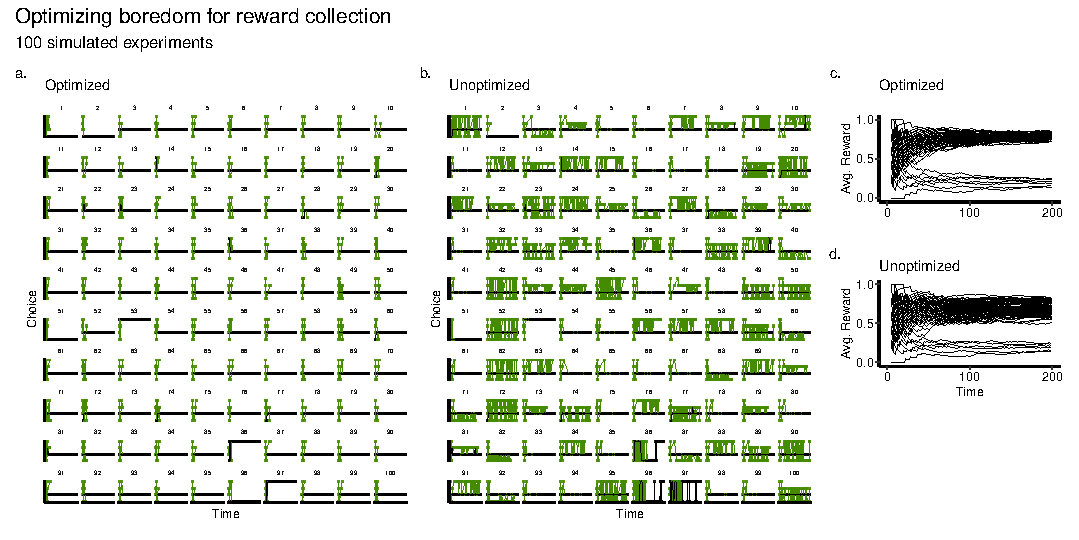
\includegraphics[width=.9\linewidth]{img/boredom2.pdf} 
	\caption{The importance of boredom during reward collection (Task 2). One hundred example experiments, each began with a different random seed. 
	\textbf{a}. Behavioral choices with optimized boredom.
	\textbf{b}. Behavioral choices with unoptimized boredom.
	\textbf{c,d}. Average reward as a function of time for optimized (c) and unoptimized (d) boredom.
	}
	\label{fig:boredom2} 
	\end{fullwidth}
\end{figure}

Unlike idealised simulations, animals cannot pre-optimize their search parameters for every task. We therefore explored reward collection as a function of 1000 randomly chosen search parameters, and reexamined performance on two tasks. These were chosen to represent an ``easy'' task, and a ``hard one''. The results are shown in Fig.~\ref{fig:robust}. 

As above exploitation by deterministic curiosity produced top-3 performance on both tasks (Fig.~\ref{fig:robust}a-b). Most interesting is the performance for the worst parameters. Here deterministic curiosity was markedly better and the other still. We can explain this in the following way. All the other exploration strategies use parameters to tune the degree of exploration. With deterministic curiosity though we tune only when exploration should stop. The degree of exploration--measure by how close it is to maximum entropy--is fixed by the model itself. And it seems that here at least it is far more robust to tune the stopping point, rather than the degree of exploration.

\begin{figure}
	\begin{fullwidth}
	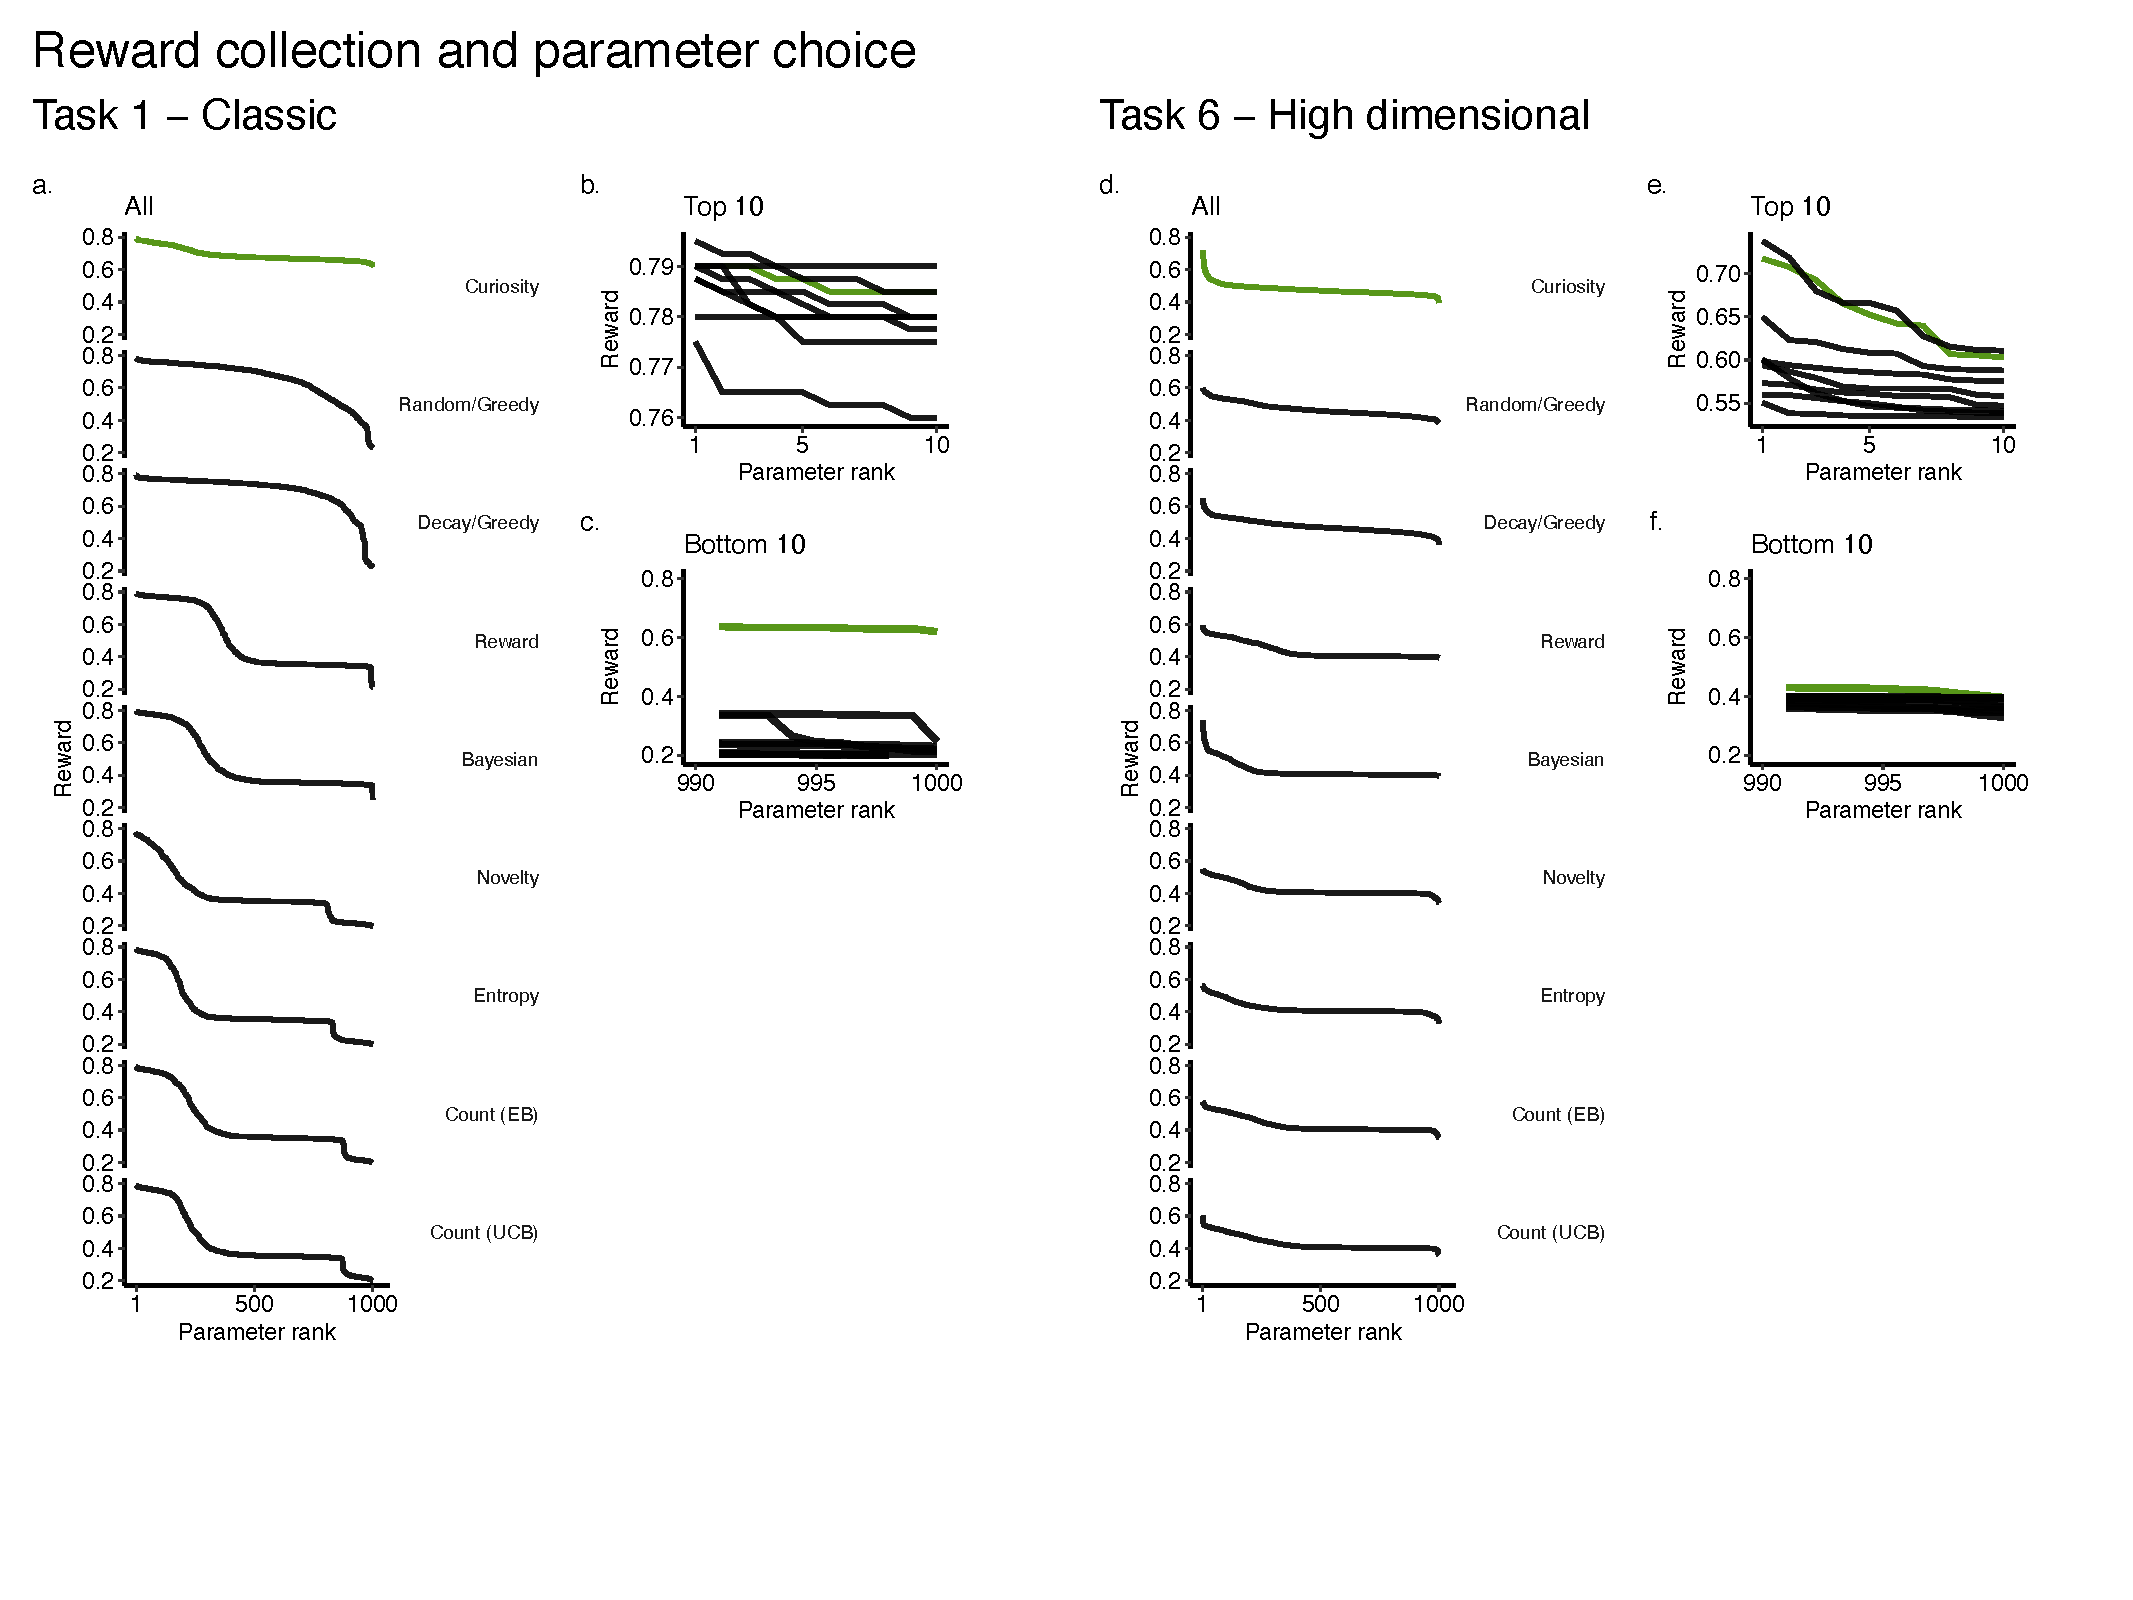
\includegraphics[width=0.8\linewidth]{img/robust.pdf} 
	\caption{Parameter selection and search performance (\textit{Task 2} and \textit{6}). We wanted to evaluate how robust performance was to poor and random hyperparameters. A very robustness exploration algorithm would produce strong performance with both the best parameter choices, and the worst parameter choices.   
	\textbf{a,d} Total reward for 1000 search hyperparameters, for each of strategies we considered.  
	\textbf{b,e} Performance with the top 10 hyperparameters, curiosity (green) compared to all the others.
	\textbf{c.f} Performance with the bottom 10 hyperparameters.
	\textbf{TODO} - add error bars
	}
	\label{fig:robust}
	\end{fullwidth}
\end{figure}

% -------
% Move to discussion
If our deterministic solution is working as the mathematics predict it should,  then adding a random aspect to either exploration or exploitation should only act to degrade performance. We showed an example of this in Fig.~\ref{fig:independent2}. Here adding two levels of random noise to the choices only served to increase variability of convergence (left) and reduce the total rewards collected (right). When we then compare performance between curiosity and the other strategies as noise smoothly changes we see performance eventually decline to chance levels. 

In studying noise in Fig ~\ref{fig:forced} many of the strategies showed a peak in performance as noise increased, suggesting a minimum level of noise is needed for satisfactory performance. There were two strategies where this was not the case: entropy and Bayesian. These showed some ability to operate well low stochasticity. If this trend when removing stochasticity completely, then that would be half of the ingredients needed to find another set of zero regret solutions. When however we ``forced'' determinism on these and other strategies, performance declined to chance (Fig ~\ref{fig:forced}b). The exception to this is the Bayesian strategy, whose median performance approaches the ideal (0.8). Hope for this exception is limited however by its having substantially more variance than any others. In other words, it appeared to be unreliable.

\begin{figure}
	\begin{fullwidth}
	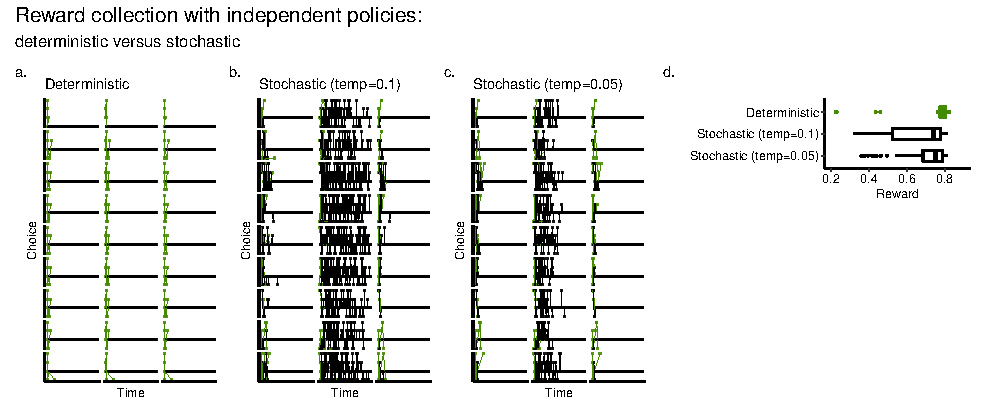
\includegraphics[width=0.6\linewidth]{img/independent2.pdf} 
	\caption{Behavior during reward collection, using either deterministic or stochastic curiosity (\textit{Task 2}). 
	\textbf{a-c} Examples of exploration choices using Eq~\ref{eq:meta_greedy}. In the left panel is the deterministic version. The other two panels show the same algorithm with two levels of noise added to both curiosity and reward collection policies. 
	\textbf{d.} The effect of noise on rewards collected, over 100 independent experiments.}
	\label{fig:independent2}
	\end{fullwidth}
\end{figure}

\begin{figure}
	\begin{fullwidth}
	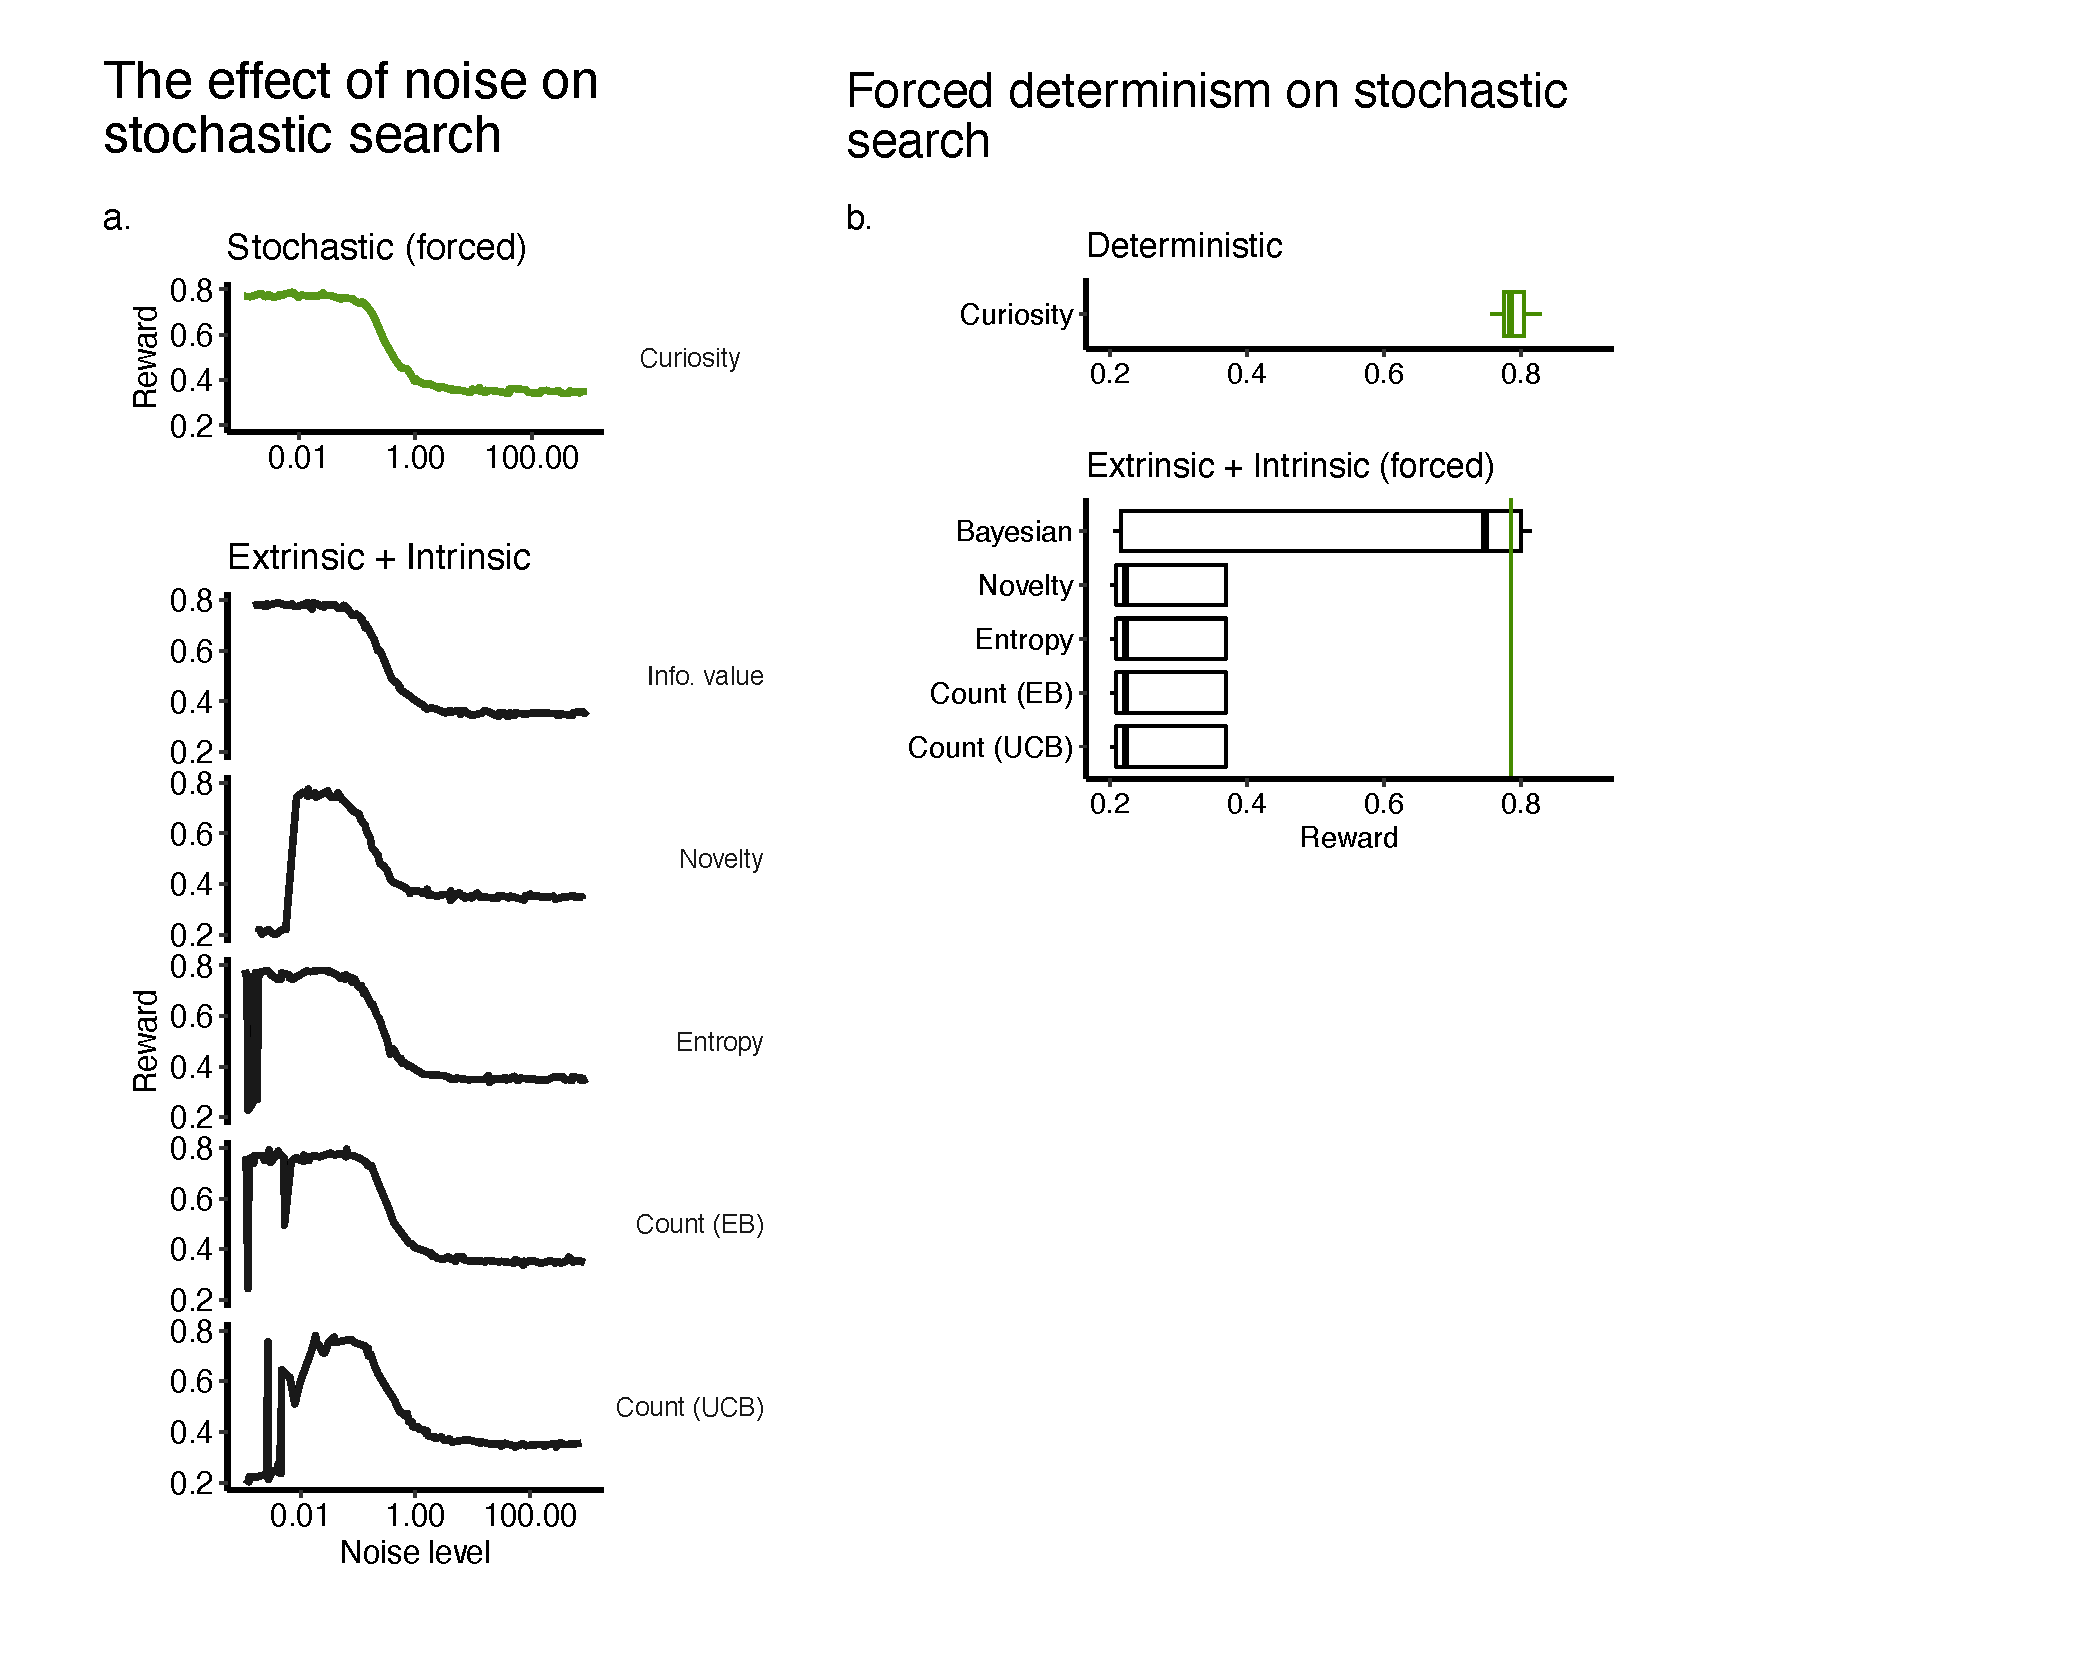
\includegraphics[width=0.6\linewidth]{img/forced.pdf} 
	\caption{Adding noise, or forcing determinism (\textit{Task 2}). 
	\textbf{a.} In this panel we forced our deterministic approach to behavior stochastically. We compared ours to all the others as the level of noise increased. \textbf{TODO} - add error bars
	\textbf{b.} In this panel we forced several of the search strategies which rely in part on stochastic search to operate in a deterministic way. We plot total reward for these agents, compared to our deterministic approach (green).
	}
	\label{fig:forced}
	\end{fullwidth}
\end{figure}


